\begin{center}
  \textbf{Exercices Théoriques - Analyse Numérique - 2017 \\
  Section MA \\
  Prof. A. Quarteroni \\
  Séance 2 - Normes matricielles et conditionnement des systèmes linéaires}
\end{center}


\vspace{10mm}

\begin{ex}
Soit $\norm{\cdot}$ une norme vectorielle. Prouver que la fonction
\begin{equation}
\label{eq:norm}
  \norm{A} = \sup_{\mathbf{x \neq 0}} \dfrac{\norm{A \BoldX}}{\BoldX}
\end{equation}

est une norme matricielle, en remarquant que la relation (\refeq{eq:norm}) est équivalente \footnote{En effet, on peut définir pour tout $\BoldX \neq 0$ un vecteur unitaire $\mathbf{u} \equiv \BoldX /\norm{\BoldX}$ de sorte que (\refeq{eq:norm}) s'écrive
\begin{equation*}
  \norm{A} = \sup_{\norm{\mathbf{u}} = 1} \norm{A \mathbf{u}} = \norm{A \mathbf{w}}
  \quad \text{avec }
  \norm{\mathbf{w}} = 1.
\end{equation*}} à

\begin{equation*}
  \norm{A} = \sup_{\norm{\BoldX} = 1} \norm{A \BoldX}.
\end{equation*}

\end{ex}

\begin{sol}
En utilisant l'astuce, on montre directement que cette définition forme une norme matricielle.

\begin{enumerate}[label=\alph*)]
  \item Si $\norm{A \BoldX} \geq 0$, alors $\norm{A} = \sup_{\norm{\BoldX} = 1} \norm{A \BoldX} \geq 0$. De plus
  
  \begin{equation*}
    \norm{A} = \sup_{\BoldX \neq \BoldZero} \dfrac{\norm{A \BoldX}}{\norm{\BoldX}} = 0
    \LRA
    \norm{A \BoldX} = 0 \ \forall \ \BoldX \neq \BoldZero,
  \end{equation*}
  
  ou encore
  
  \begin{equation*}
    A \BoldX = 0 \ \forall \ \BoldX \neq \BoldZero
    \LRA
    A = \BoldZero.
  \end{equation*}
  
  Donc, $\norm{A} = 0 \LRA A = \BoldZero$.
  
  \item Soit un scalaire $\alpha$, on a 
  
  \begin{equation*}
    \norm{\alpha A}
    = \sup_{\norm{\BoldX} = 1} \norm{\alpha A \BoldX}
    = \abs{\alpha} \sup_{\norm{\BoldX} = 1} \norm{A \BoldX}
    = \abs{\alpha} \norm{A}.
  \end{equation*}
  
  \item Vérifions enfin l'inégalité triangulaire. Par définition du supremum, si $\BoldX \neq \BoldZero$ alors
  
  \begin{equation*}
    \dfrac{\norm{A \BoldX}}{\norm{\BoldX}} \leq \norm{A}
    \Rightarrow \norm{A \BoldX} \leq \norm{A} \norm{\BoldX},
  \end{equation*}
  
  ainsi, en prenant $\BoldX$ de norme 1, on obtient
  
  \begin{equation*}
    \norm{\parent{A + B} \BoldX}
    \leq \norm{A \BoldX} + \norm{B \BoldX}
    \leq \norm{A} + \norm{B}, 
  \end{equation*}
  
  d'où on déduit $\norm{A + B} = \sup_{\norm{\BoldX} = 1} \norm{\parent{A + B} \BoldX} \leq \norm{A} + \norm{B}$.
  
  
  
\end{enumerate}




\end{sol}

\begin{ex}
Soit $\triple{\cdot}$ une norme matricielle subordonnée à une norme vectorielle $\norm{\cdot}$.
Prouver que

\begin{enumerate}[label=\alph*)]
  \item $\norm{A \BoldX} \leq \triple{A} \norm{\BoldX}$, i.e. $\triple{\cdot}$ est une norme compatible (ou consistante) avec $\norm{\cdot}$ ;
  \item $\triple{I} = 1$ ;
  \item $\triple{A B} \leq \triple{A} \triple{B}$, i.e. $\triple{\cdot}$ est sous-multiplicative.
\end{enumerate}
\end{ex}

\begin{sol}
\begin{enumerate}[label=\alph*)]
  \item Par définition du supremum, si $\BoldX \neq \BoldZero$ alors
  
  \begin{equation*}
    \triple{A} = \sup_{\BoldY \neq \BoldZero} \dfrac{\norm{A \BoldY}}{\norm{\BoldY}}
    \geq \dfrac{\norm{A \BoldX}}{\norm{\BoldX}}
    \Rightarrow 
    \norm{A \BoldX} \leq \triple{A} \norm{\BoldX}.
  \end{equation*}
  
  \item Par la définition de la norme matricielle subordonnée à une norme vectorielle
  
  \begin{equation*}
    \triple{I} = \sup_{\BoldX \neq \BoldZero} \dfrac{\norm{I \BoldX}}{\norm{\BoldX}} = 1.
  \end{equation*}
  
  \item Par la compatibilité de la norme, on déduit
  
  \begin{equation*}
    \triple{A B}
    = \sup_{\norm{\BoldX} = 1} \norm{A B \BoldX}
    \leq \sup_{\norm{\BoldX} = 1} \triple{A} \norm{B \BoldX}
    = \triple{A} \sup_{\norm{\BoldX} = 1} \norm{B \BoldX}
    = \triple{A} \triple{B}.
  \end{equation*}
  
\end{enumerate}
\end{sol}

\begin{ex}
Montrer que, si $\norm{\cdot}$ est une norme matricielle consistante avec une norme vectorielle $\norm{\cdot}$, alors $\rho \parent{A} \leq \norm{A} \ \forall \ A \in \C^{n \times n}$.
\end{ex}

\begin{sol}
Si $\lambda$ est une valeur propre de $A$, alors il existe $\BoldV \neq \BoldZero$, vecteur propre de $A$, tel que $A \BoldV = \lambda \BoldV$.
Ainsi, puisque $\norm{\cdot}$ est consistante,

\begin{equation*}
  \abs{\lambda} \norm{\BoldV}
  = \norm{\lambda \BoldV}
  = \norm{A \BoldV}
  \leq \norm{A} \norm{\BoldV}
\end{equation*}

et donc $\abs{\lambda} \leq \norm{A}$.
Cette inégalité étant vraie pour toute valeur propre de $A$, elle l'est en particulier quand $\abs{\lambda}$ est égale au rayon spectral.
\end{sol}

\begin{ex}
Étant donnée la matrice $A \in \R^{2 \times 2}$, $a_{11} = a_{22} = 1$, $a_{12} = \gamma$, $a_{21} = 0$, vérifier que pour $\gamma \geq 0$, $K_{\infty} \parent{A} = K_{1} \parent{A} = \parent{1 + \gamma}^{2}$.
Soit $A \BoldX = \BoldB$ le système linéaire où $\BoldB$ est tel que $\BoldX = \parent{1 - \gamma, 1}^{\top}$ soit la solution.
Trouver une majoration du type 

\begin{equation*}
  \dfrac{\norm{\delta \BoldX}_{\infty}}{\norm{\BoldX}_{\infty}}
  \leq C \dfrac{\norm{\delta \BoldB}_{\infty}}{\norm{\BoldB}_{\infty}}
\end{equation*}

avec $C > 0$ une constante qui ne dépend que de $\norm{A^{-1}}_{\infty}$, $\norm{\BoldB}_{\infty}$ et $\norm{\BoldX}_{\infty}$.
Le vecteur $\parent{\BoldX + \delta \BoldX}$ est la solution du système perturbé $A \parent{\BoldX + \delta \BoldX} = \parent{\BoldB + \delta \BoldB}$ avec $\delta \BoldB$ une perturbation du vecteur $\BoldB$.
Le problème est-il bien conditionné par rapport à $\gamma \rightarrow \infty$ ?
\end{ex}

\begin{sol}
On a 

\begin{equation*}
  A = \begin{bmatrix}
        1 & \gamma  \\
        0 & 1
      \end{bmatrix}
  , \quad
  A^{-1} = \begin{bmatrix}
        1 & - \gamma  \\
        0 & 1
      \end{bmatrix}.
\end{equation*}

Ainsi, puisque $\gamma \geq 0$,

\begin{gather*}
  \norm{A}_{1} = \max_{j = 1, 2} \sum_{i = 1}^{2} \abs{a_{ij}} = \max \bracket{1, 1 + \gamma} = 1 + \gamma, \\
  \norm{A}_{\infty} = \max_{i = 1, 2} \sum_{j = 1}^{2} \abs{a_{ij}} = \max \bracket{1 + \gamma, 1} = 1 + \gamma, \\
  \norm{A^{-1}}_{1} = \max \bracket{1, 1 + \gamma} = 1 + \gamma, \\
  \norm{A^{-1}}_{\infty} = \max \bracket{1 + \gamma, 1} = 1 + \gamma.
\end{gather*}

Par conséquent,

\begin{equation*}
  K_{1} \parent{A}
  = \norm{A}_{1} \norm{A^{-1}}_{1} 
  = K_{\infty} \parent{A}
  = \norm{A}_{\infty} \norm{A^{-1}}_{\infty}
  = \parent{1 + \gamma}^{2}. 
\end{equation*}

On a

\begin{equation*}
  \BoldB = A \BoldX = \begin{bmatrix}
        1   \\
        1
      \end{bmatrix},
\end{equation*}

en particulier $\norm{\BoldB}_{\infty} = 1$. 
En perturbant le second membre du système $A \BoldX = \BoldB$ (on ne perturbe pas la matrice), on obtient un système perturbé de la forme

\begin{equation*}
  A \parent{\BoldX + \delta \BoldX} = \BoldB + \delta \BoldB,
\end{equation*}

donc

\begin{equation*}
  \delta \BoldX = A^{-1} \delta \BoldB.
\end{equation*}

On en tire que 

\begin{equation*}
  \norm{\delta \BoldX}_{\infty}
  \leq \norm{A^{-1}}_{\infty} \norm{\delta \BoldB}_{\infty}.
\end{equation*}

En divisant par $\norm{\BoldX}_{\infty}$, on trouve 

\begin{equation*}
  \dfrac{\norm{\delta \BoldX}_{\infty}}{\norm{\BoldX}_{\infty}}
  \leq \dfrac{\norm{A^{-1}}_{\infty}}{\norm{\BoldX}_{\infty}} \norm{\delta \BoldB}_{\infty}.
\end{equation*}

En plus, puisque $\norm{\BoldB}_{\infty} = 1$, on peut écrire

\begin{equation*}
  \dfrac{\norm{\delta \BoldX}_{\infty}}{\norm{\BoldX}_{\infty}}
  \leq \underbrace{\dfrac{\norm{A^{-1}}_{\infty}}{\norm{\BoldX}_{\infty}}}_\text{$C$}
  \dfrac{\norm{\delta \BoldB}_{\infty}}{\norm{\BoldB}_{\infty}}
\end{equation*}

avec $C = \dfrac{\norm{A^{-1}}_{\infty}}{\norm{\BoldX}_{\infty}}$ la constante cherchée.
On a donc que 

\begin{equation*}
  C = \dfrac{1 + \gamma}{\max \bracket{1, \abs{1 - \gamma}}}.
\end{equation*}

On voit bien que $C \rightarrow 1$ quand $\gamma \rightarrow \infty$.
Ainsi, pour le cas particulier de $\BoldB = \parent{1, 1}^{\top}$, le problème est bien conditionné.
Remarquons que, dans le cas général ($\BoldB$ arbitraire), le problème est mal conditionné pour $\gamma$ grand.
En effet, $K_{\infty} \parent{A} \rightarrow \infty$ quand $\gamma \rightarrow \infty$.
Cet exercice met en évidence que le fait d'avoir une matrice avec un grand conditionnement n'empêche pas nécessairement le système global d'être bien conditionné pour des choix particuliers du second membre $\BoldB$.












\end{sol}

\begin{ex}
Supposons que $\norm{\delta A} \leq \gamma \norm{A}$, $\norm{\delta \BoldB} \leq \gamma \norm{\BoldB}$ avec $\gamma \in \R^{+}$ et $\delta A \in \R^{n \times n}$, $\delta \BoldB \in \R^{n}$.
On veut montrer que, si $\gamma K \parent{A} < 1$, on a les inégalités suivantes :

\begin{equation}
\label{eq:xPlusDelta}
  \dfrac{\norm{\BoldX + \delta \BoldX}}{\norm{\BoldX}}
  \leq \dfrac{1 + \gamma K \parent{A}}{1 - \gamma K \parent{A}},
\end{equation}

\begin{equation}
\label{eq:xDelta}
  \dfrac{\norm{\delta \BoldX}}{\norm{\BoldX}}
  \leq \dfrac{2 \gamma}{1 - \gamma K \parent{A}} \ K \parent{A}.
\end{equation}

\begin{enumerate}[label=\alph*)]
  \item Si $C$ est une matrice carrée telle que $\rho \parent{C} < 1$, on sait (voir le Théorème 1.5 du livre) que $I - C$ est inversible.
        Montrer que dans ce cas on a
        
        \begin{equation}
        \label{eq:normC}
          \dfrac{1}{1 + \norm{C}}
          \leq \norm{\parent{I - C}^{-1}}
          \leq \dfrac{1}{1 - \norm{C}}.
        \end{equation}
        
        où $\norm{\cdot}$ est est une norme matricielle subordonnée à une norme vectorielle telle que $\norm{C} \leq 1$. 
        
        \item Montrer l'inégalité (\refeq{eq:xPlusDelta}) en utilisant le résultat du point 1 et le fait que $\parent{A + \delta A} \parent{\BoldX + \delta \BoldX} = \BoldB + \delta \BoldB$.
        
        \item Montrer l'inégalité (\refeq{eq:xDelta}). Suggestion: utiliser l'inégalité triangulaire $\norm{\BoldX + \delta \BoldX} \leq \norm{\BoldX} + \norm{\delta \BoldX}$.

\end{enumerate}



\end{ex}

\begin{sol}
\begin{enumerate}[label=\alph*)]
  \item Puisque \footnote{On suppose (toujours) que $\norm{\cdot}$ est une norme matricielle subordonnée à une norme vectorielle.} $\norm{I} = 1$, on a (Exercice 2, Série 2)
  
  \begin{equation*}
    1 = \norm{I}
    \leq \norm{I - C} \norm{\parent{I - C}^{-1}}
    \leq \parent{1 + \norm{C}} \norm{\parent{I - C}^{-1}},
  \end{equation*}
  
  ce qui donne la première égalité de (\refeq{eq:normC}).
  Pour la seconde, en remarquant que $I = I - C + C$ et en multipliant à droite les deux membres par $\parent{I - C}^{-1}$, on a $\parent{I - C}^{-1} = I + C \parent{I - C}^{-1}$.
  En prenant les normes, on obtient
  
  \begin{equation*}
    \norm{\parent{I - C}^{-1}} \leq 1 + \norm{C} \norm{\parent{I - C}^{-1}},
  \end{equation*}
  
  d'où on déduit la seconde inégalité, puisque $\norm{C} < 1$.
  
  \item Soit
  
  \begin{equation*}
    \parent{A + \delta A} \parent{\BoldX + \delta \BoldX} = \BoldB + \delta \BoldB.
  \end{equation*}
  
  Alors, on a
  
  \begin{equation*}
    \parent{I + A^{-1} \delta A} \parent{\BoldX + \delta \BoldX} = \BoldX + A^{-1} \delta \BoldB.
  \end{equation*}
  
  De plus, puisque $\gamma K \parent{A} < 1$ et $\norm{\delta A} \leq \gamma \norm{A}$ on a 
  
  \begin{equation*}
    \norm{A^{-1} \delta A}
    \leq \norm{A^{-1}} \norm{\delta A}
    \leq \gamma \norm{A^{-1}} \norm{A}
    = \gamma K \parent{A} < 1.
  \end{equation*}
  
  Alors, $\rho \parent{A^{-1} \delta A} < 1$ et $I + A^{-1} \delta A$ est inversible.
  En prenant l'inverse de cette matrice et en passant aux normes, on obtient
  
  \begin{equation*}
    \norm{\BoldX + \delta \BoldX}
    \leq \norm{\parent{I + A^{-1} \delta A}^{-1}} \parent{\norm{\BoldX} + \gamma \norm{A^{-1}} \norm{\BoldB}}.
  \end{equation*}
  
  Alors, l'inégalité du point 1 donne 
  
  \begin{equation*}
    \norm{\BoldX + \delta \BoldX}
    \leq \dfrac{1}{1 - \norm{A^{-1} \delta A}} \parent{\norm{\BoldX} + \gamma \norm{A^{-1}} \norm{\BoldB}},
  \end{equation*}
  
  ce qui implique
  
  \begin{equation*}
    \dfrac{\norm{\BoldX + \delta \BoldX}}{\norm{\BoldX}}
    \leq \dfrac{1 + \gamma K \parent{A}}{1 - \gamma K \parent{A}},
  \end{equation*}
  
  puisque $\norm{A^{-1} \delta A} \leq \gamma K \parent{A}$ et $\norm{\BoldB} \leq \norm{A} \norm{\BoldX}$.
  
  \item Montrons à présent que l'inéquation (\refeq{eq:xDelta}) est correcte.
  En retranchant $A \BoldX = \BoldB$ de \eqref{eq:xPlusDelta}, on a 
  
  \begin{equation*}
    A \delta \BoldX = - \delta A \parent{\BoldX + \delta \BoldX} + \delta \BoldB.
  \end{equation*}
  
  En prenant l'inverse de $A$ et en passant aux normes, on obtient l'inégalité suivante 
  
  \begin{equation*}
    \begin{split}
      \norm{\delta \BoldX}
      & \leq \norm{A^{-1} \delta A} \norm{\BoldX + \delta \BoldX} + \norm{A^{-1}} \norm{\delta \BoldB} \\
      & \leq \gamma K \parent{A} \norm{\BoldX + \delta \BoldX} + \gamma \norm{A^{-1}} \norm{\BoldB}
    \end{split}
  \end{equation*}
  
  En divisant les deux membres par $\norm{\BoldX}$ et en utilisant l'inégalité triangulaire $\norm{\BoldX + \delta \BoldX} \leq \norm{\BoldX} + \norm{\delta \BoldX}$, on obtient finalement (\refeq{eq:xDelta}).
  
  
\end{enumerate}
\end{sol}

\begin{ex}
\begin{enumerate}[label=\alph*)]
  \item Soit $A \in \R^{n \times n}$ une matrice symétrique définie positive et soient $\lambda_{i}$ et $\BoldV_{i}$, $i = 1, \dots, n$, les valeurs propres et les vecteurs propres de $A$.
  Montrer que si $\BoldX$ est la solution du système linéaire $A \BoldX = \BoldB$, alors

  \begin{equation*}
    \BoldX = \sum_{i = 1}^{n} \parent{c_{i} / \lambda_{i}} \BoldV_{i},
  \end{equation*}

  où $c_{i}$ est la $i$-ème composante de $\BoldB$ dans la base des vecteurs propres de $A$.
  
  \item On se donne maintenant le système linéaire $A \BoldX = \BoldB$ suivant
  
  \begin{equation*}
        \begin{bmatrix}
          1001 & 1000  \\
          1000 & 1001
        \end{bmatrix}
        \cdot
        \begin{bmatrix}
          x_{1}   \\
          x_{2} 
        \end{bmatrix}
        =
        \begin{bmatrix}
          b_{1}   \\
          b_{2} 
        \end{bmatrix}
        \quad 
        ,
  \end{equation*}
  
  où $A$ est mal-conditionnée avec les valeurs propres $\lambda_{1} = 1, \lambda_{2} = 2001$.
  En décomposant le second membre sur la base des vecteurs propres de la matrice $A$, expliquer pourquoi, lorsque $\BoldB = \parent{2001, 2001}^{\top}$, une petite perturbation $\delta \BoldB = \parent{1, 0}^{\top}$ produit de grandes variations dans la solution, et réciproquement, si $\BoldB = \parent{1, -1}^{\top}$, une petite variation $\delta \BoldX = \parent{0.001, 0}^{\top}$ dans la solution induit de grandes variations dans $\BoldB$.
  
  
\end{enumerate}


\end{ex}

\begin{sol}
\begin{enumerate}[label=\alph*)]
  \item Puisque $A$ est une matrice symétrique, il existe une matrice $V$ orthogonale et une matrice $D$ diagonale dont tous les coefficients sont réels, telles que
  
  \begin{equation*}
    V^{-1} A V = D = \text{diag} \bracket{\lambda_{1}, \dots, \lambda_{n}}
  \end{equation*}
  
  ou, de façon équivalente, $A \BoldV_{i} = \lambda_{i} \BoldV_{i}$ pour $i = 1, \dots, n$, de sorte que les vecteurs colonnes de $V$ soient les vecteurs propres de $A$.
  De plus, les vecteurs propres sont deux à deux orthogonaux (et peuvent être normalisés : donc, on a que $\BoldV_{j}^{\top} \BoldV_{l} = \delta_{jl}$, où $\delta_{jl}$ est le symbole de Kronecker) et on déduit que les vecteurs propres d'une matrice symétrique sont orthogonaux et engendrent l'espace $\R^{n}$ tout entier.


  Donc, soient $\BoldB = \sum_{i = 1}^{n} c_{i} \BoldV_{i}$ le membre de droite du système linéaire $A \BoldX = \BoldB$ et $\BoldX$ sa solution ; en écrivant aussi $\BoldX$ dans la base des vecteurs propres de $A$, on a :
  
  \begin{equation*}
    A \BoldX
    = A \sum_{i = 1}^{n} x_{i} \BoldV_{i} 
    = \sum_{i = 1}^{n} c_{i} \BoldV_{i}.
  \end{equation*}
  
  Et, puisque $A \BoldV_{i} = \lambda_{i} \BoldV_{i}$, on trouve
  
  \begin{equation*}
    \sum_{i = 1}^{n} x_{i} \lambda_{i} \BoldV_{i} 
    = \sum_{i = 1}^{n} c_{i} \BoldV_{i}.
  \end{equation*}
  
  Donc on trouve
  
  \begin{equation*}
    \sum_{i = 1}^{n} \parent{\lambda_{i} x_{i} - c_{i}} \BoldV_{i} 
    = 0,
  \end{equation*}
  
  c'est-à-dire $\lambda_{i} x_{i} = c_{i}$ et
  
  \begin{equation*}
    \BoldX = \sum_{i = 1}^{n} \parent{c_{i} / \lambda_{i}} \BoldV_{i}.
  \end{equation*}
  
  
  \item Les vecteurs propres de la matrice $A$ sont $\BoldV_{1} = \parent{1, -1}^{\top}$ (qui correspond à $\lambda_{1} = 1$) et $\BoldV_{2} = \parent{1, 1}^{\top}$ (qui correspond à $\lambda_{2} = 2001$).
  Soit $\BoldB = \parent{2001, 2001}^{\top}$ et $\delta \BoldB = \parent{1, 0}^{\top}$.
  Alors,
  
  \begin{equation*}
    \BoldB + \delta \BoldB
    =   \begin{bmatrix}
          2001 \\
          2001
        \end{bmatrix} 
        +
        \begin{bmatrix}
          1 \\
          0
        \end{bmatrix} 
    = 2001 \BoldV_{2} + \dfrac{1}{2} \parent{\BoldV_{1} + \BoldV_{2}}
    = \dfrac{1}{2} \BoldV_{1} + \dfrac{4003}{2} \BoldV_{2}.
  \end{equation*}
  
  Si on écrit la solution $\BoldX$ comme combinaison linéaire des vecteurs propres, on trouve
  
  \begin{equation*}
    \BoldX
    = \dfrac{\frac{1}{2}}{1} \BoldV_{1} + \dfrac{\frac{4003}{2}}{2001} \BoldV_{2}
    = \dfrac{1}{2} \BoldV_{1} + \dfrac{4003}{4002} \BoldV_{2}
    \approx 
    \begin{bmatrix}
      1.5 \\
      0.5
    \end{bmatrix}. 
  \end{equation*}
  
  Ainsi on voit que l'erreur $\delta \BoldX$ par rapport à la solution exacte $\BoldX = \parent{1, 1}^{\top}$ est $\delta \BoldX \approx \parent{0.5, -0.5}^{\top}$.
  
  Réciproquement, soit $\BoldB = \parent{1, -1}^{\top}$. La solution exacte du système est $\BoldX = \parent{1, -1}^{\top}$.
  On exprime la solution perturbée par rapport aux vecteurs propres :
  
  \begin{equation*}
    \BoldX + \delta \BoldX
    =   \begin{bmatrix}
          1.001 \\
          -1
        \end{bmatrix} 
    = \dfrac{2.001}{2} \BoldV_{1} + \dfrac{0.001}{2} \BoldV_{2},
  \end{equation*}
  
  d'où $c_{1} = 2.001/2$ et $c_{2} = 0.001/2$. Donc 
  
  \begin{equation*}
    \BoldB + \delta \BoldB
    =   \begin{bmatrix}
          2.001 \\
          0
        \end{bmatrix} 
  \end{equation*}
  
  et $\delta \BoldB = \parent{1.001, 1}^{\top}$.
  
  \textit{Remarque.}
  Le système linéaire de cet exercice pourrait être obtenu de l'analyse d'une barre rigide attachée dans sa partie central à un ressort de raideur 4000 et connectée aux extremités à deux ressorts de raideur 1 (voir Figure \ref{fig:ressort} ci-dessous).
  On applique des forces $b_{1}$ et $b_{2}$ aux extremités de la barre et on observe ses déplacements verticaux $x_{1}$ et $x_{2}$.
  Si les forces $b_{1}$ et $b_{2}$ sont équilibrées (par exemple $b_{1} = 2001$, $b_{2} = 2001$), alors de petits changements $\delta \BoldB$ engendrent des mouvements significatifs de la barre (grand $\delta \BoldX$).
  A l'inverse, si les forces ne sont pas équilibrées (par exemple $b_{1} = 1$, $b_{2} = -1$), alors on peut obtenir de petits déplacements $\delta \BoldX$ même si on impose de forts changements $\delta \BoldB$ sur les forces exercées.
  
  \begin{figure}[h!]
    \centering
    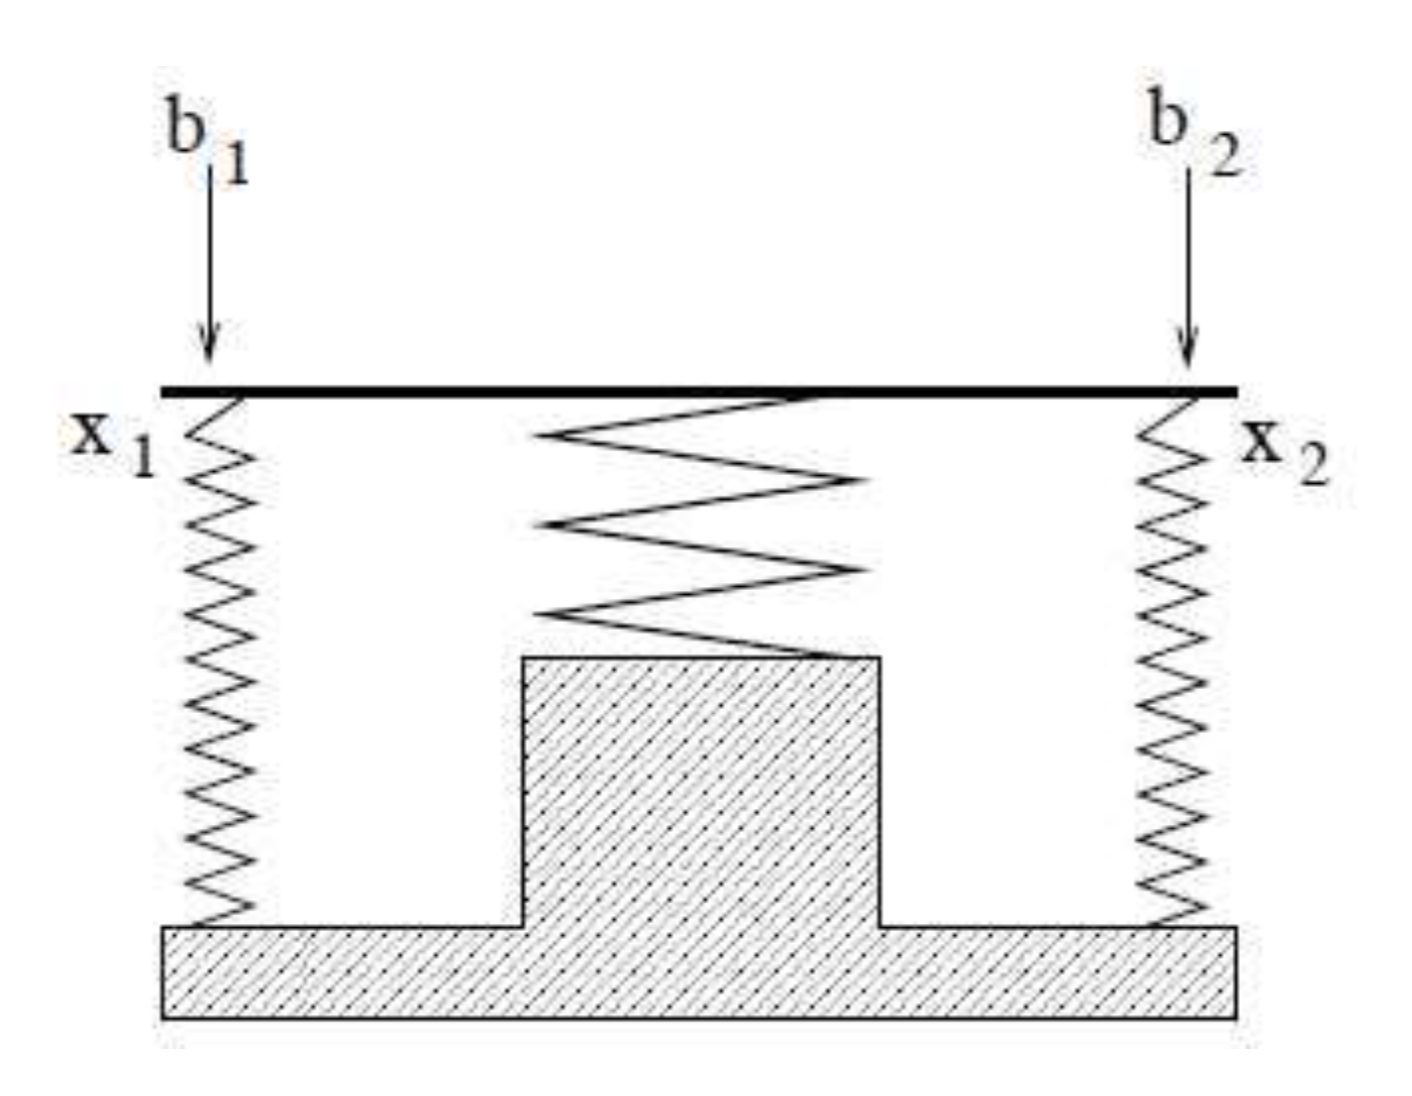
\includegraphics[scale = 0.2]{s2/images/ressort.png}
    \caption{Ressort}
    \label{fig:ressort}
  \end{figure}


\end{enumerate}





\end{sol}




